%
%  $Author: awl8049 $
%  $Date: 2011/11/16 08:28:50 $
%  $Revision: 3.1 $
%
%\documentclass[times, 10pt,twocolumn]{article} 
\documentclass[times, 10pt,onecolumn]{article} 
\usepackage{setspace}
\usepackage{latex8}
\usepackage{graphicx}
\usepackage{authblk}
\usepackage{amsmath}
\usepackage{amsthm}
%\usepackage{pdfsync}
\pagestyle{plain}
\begin{document}
\title{Run-time Energy Consumption Estimation Based On Workload in
  Server Systems}
\author[*]{}
\author[*]{Adam Lewis} 
\author[*]{Soumik Ghosh} 
\author[*]{N.-F. Tzeng}
\affil[*]{Center for Advanced Computer Studies\\ 
 University of Louisiana at Lafayette\\ 
 Lafayette, LA 70504, USA\\ 
 \{awlewis,sxg5317,tzeng\}@cacs.louisiana.edu
}
\maketitle
\newtheorem{defn}{Definition}
\newtheorem{thm}{Theorem}
\thispagestyle{empty}
\doublespacing

\begin{abstract}
  The upwardly spiraling operating costs of the infrastructure for
  enterprise-scale computing demand efficient power management in server
  environments.  This is difficult to achieve in practice as a data
  center usually over-provisions its power capacity to address the worst
  case scenarios. This often results in either waste of considerable
  power budget or severe underutilization of capacity.  Thus, it is
  critical to quantitatively understand power consumption at the system
  level to optimize the use of deployed power capacity in the data
  center.

  This paper introduces an analytical model that provides run-time
  system-wide prediction of power consumption on server blades.  The
  model takes into account key aspects of system power consumption from
  power supplies to processor workload in order to control the die
  temperatures and the ambient temperature for regulating system energy
  consumption within a given power and thermal envelope.

  Previous work using hardware performance counters for system power
  estimation proposes techniques to estimate system and subsystem static
  power consumption.  In contrast, we demonstrate a method for run-time
  system power estimation that dynamically correlates system-bus traffic
  with task activities, memory-access metrics and board-level power
  measurements.  Using the HyperTransport bus model as a case study and
  through electrical measurements on example server subsystems, we
  develop a statistical model for this run-time power computation.  We
  suggest possible scheduler-based mechanisms to take advantage of this
  estimation model when dispatching jobs to confine server power
  consumption within power budget and thermal envelope while maximizing
  system throughput.
\end{abstract}

\section{Introduction}
\label{sec:Introduction}
The heart of the infrastructure of today's information economy is the
data centers containing the servers that support most Internet services.
Such centers host hundreds or even thousands of servers running
off-the-shelf hardware.  The power demands of these installations force
firms to install complex and costly cooling solutions to efficiently
move the heat away from servers so as to avoid reliability problems.

Providing proper cooling has become more difficult as the density of the
off-the-shelf hardware has increased with tighter packaging, decreasing
form factors, and increasing performance demands.  The introduction of
multi-core processors combined together in clusters of traditional and
blade servers has greatly increased the power demands of servers.

Server systems, per \cite{Bianchini2004}, have characteristics that make
traditional power management techniques undesirable:
\begin{itemize}
\item server hardware is typically provisioned for peak load, and thus
  exhibit high performance and power consumption;
\item high availability and high bandwidth is typically provided by widespread
  replication of resources such as clusters of machine and disk arrays;
\item server power supplies must be able to store capacity to deal with sudden
  spikes in load and as result exhibit high power losses.
\end{itemize}

Application servers pose an especially interesting power management problem due
to intensive CPU and memory requirements combined with maintaining soft state
that is not typically replicated.   Intensive CPU and memory use means that
traditional power management mechanisms may impose too excessive demands upon
performance while non-replicated state forces state migration in order to turn
application servers on and off.

Extensive study of the power profiles of the Intel Pentium architecture
has occured at the workstation \cite{Isci2003a} \cite{Isci2003b}
\cite{Isci2006} and server \cite{Bircher2004} \cite{Bircher2007}
\cite{Lee2005}.  However, very little consideration has been given to
the power profiles of servers constuctued using the {NUMA}-based
architecture used on processors such as the AMD64 family of processors
\cite{AMD2007}.  In contrast
to processors using a traditional frontside bus to communicate with the
outside world, these processors use a HyperTransport (HT) based bus
\cite{HT2007} to communicate between processors and the outside world.

This work contributes the following that can be used with NUMA-based processor
to create an energy-proportional server:
\begin{itemize}
\item A statistical full-system model of the power consumption of a
  NUMA-based processor that combines processor and motherboard sensor
  data, data collected with through the out-of-band management
  controller, and performance counter information collected from the
  system processor to model power.
\item A detailed experimental study of the model 
\item Power prediction software that works in conjunction with the
  operating system kernel to predict when the system needs to scale back
  voltage or frequency to reduce the power consumption on the individual server.
\end{itemize}

The remainder of this paper is structured as follows: section
\ref{sec:related} describes related work.  Section \ref{sec:model}
describes the structure of the model.  Section \ref{sec:experiment}
shows our experimental results.  Section \ref{sec:conclusions} offers
our conclusions.

\section{Related Work}
\label{sec:related}
Power management techniques developed for mobile and desktop computers have
been applied with some sucess to managing the power consumption of
microprocessors used in server hardware.  A common approach is the
application of dynamic voltage scaling: reducing the voltage (and as a
result, the frequency) of the processor at the cost of slower program
execution. Other approaches such as the approach taken by Intel with the
Pentium 4 processor have utilized a stop-go approach: activate and
deactivate the processor as demanded by workload.  These approaches have
mostly been applied most often to battery-powered devices.  They adjust
components to lowest power-mode that does not over-compromise
performance.  These transitions occur based on analysis of workload or
higher-level operation.

Work done for battery-powered laptops has been adapted for use in
consumer desktop workstations \cite{APM1994}\cite{ACPI2006}.  The
current generation of systems supports the ACPI standard
\cite{ACPI2006}.  The standard introduced the concepts of CPU, Device,
and Processor States.  These are combined into a set of up to 16
implementation specific Performance States. Processor vendors have
different implementations with the Intel SpeedStep \cite{Intel2006} and
AMD PowerNow! \cite{AMD2006} be the most prevalent in industry.

An examination of server activity patterns \cite{Fan2007}\cite{Barroso2007}
shows that servers are rarely completely idle and seldom operate near their
maximum utilization.   Analysis of server traces indicate that this behavior
is a result of two factors: the need to provision servers for the worst case
and the fact that application factors prevent extensive idle time on servers.
For Internet workloads, quality of service requirements mean that sufficient
slack be provided for the server to deal with potential server faults.
Furthermore, servers rarely become completely idle.   Data is distributed
across all servers in the server farm meaning that the server cannot become
completely idle if the data must always be available.  

Extensive study has been done on limiting the power consumption of
storage devices \cite{Pinheiro2004} and main memory \cite{Diniz2007}.
These approaches focus on these devices as the greatest energy consumers
in the system after the processor.  However, these approaches optimize
only one part of the system.  This is problematic because the system
compoenents interact with other and focusing on just one piece of the
energy consumption model may not be optimal from the standpoint of the
complete system.  An effective power model must take in account the
impact of these interactions.

The power model must also take thermal issues into account.  Management
of thermal issues is complicated by processors with multiple cores per
processor.  Power management operates on a per processor paper  An analysis
of the impact of multi-core processors can be found
in \cite{Donald2006}. 

Effective power modeling requires the use of a full-system approach.
How this is done falls into two schools of thought: modeling the power
at the simulation level, or attempting to correlating power consumption
to system-level metrics (at either the user or kernel level of the
operating system).

Power modeling through simulation using systems such as Wattach
\cite{Brooks2000} and HotSpot
\cite{Skadron2004} can provide detailed analysis and breakdown across
components in a system.    Simulation techniques have both speed and
scale issues.  Simulators are slow compared to the real hardware and do
not scale very well to long-running applications and large
data-sets. They are not an effective solution when real-time prediction
and dynamic optimization is required.

Another approach is to coorelate power consumption to phases of
application execution using system-level metrics.  The approaches used
to define this mapping fall into two categories: determining the
application phase using from either the control flow of the application
\cite{Hu2005} \cite{Iyer2001} \cite{Sherwood2003} or from performance
counter signatures of the executed instructions or operating system
metrics \cite{Bellosa2003} \cite{Isci2003a} \cite{Isci2003b}
\cite{Contreras2005} \cite{Economou2006}.  Attempts have been made to
reconcile these approaches by attempting to map programs phases to
events \cite{Isci2006}.

Models based on performance counter events and/or operating system
metrics are based on linear regression techniques where the authors
attempt to map a linear model of the collected metrics to the energy
consumed during the execution of a program 
 \cite{Isci2003c} \cite{Contreras2005}\cite{Bircher2007}.  

\section{The Model}
\label{sec:model}
In our model development procedure, we consider a single server blade
considered as a closed black-box system.  The
black-box system model lets us converge upon an upper bound of thermal, energy, and
power envelopes of the system.  We develop our model by measuring the 
energy input into the system as a function of the work done by the system in 
executing its computational tasks and the residual thermal energy given off by the system 
in doing that work. It is important to note that we
are trying to establish an energy relationship between the workload and
the overall thermodynamics of the system. 

%A major component in this
%context is, in addition to the terms in Equation \ref{eq:linmodel}, is
%the power supply in the server chassis.

We start by considering the type of power supplied into the system.
Most server blades operate on an AC input. We have considered 120 VAC
input for our experimental platform, the Sun Fire X2200 server.  The
output from the power converter in this system consists of several DC
power domains supplying power to different components in the server.
Typically, on most server systems these would +/-12Vdc, +/-5Vdc, and
+/-3.3Vdc lines.  In the case of the Sun server used in this study, two
12 Vdc lines supply power to the processor's hard drive(s) and cooling
fans in the system The 5 Vdc and 3.3 Vdc lines are dediciated to
supplying power to the support chips and perpherials on the board.  Most
switched mdoe power supplies for servers have a power conversion
efficiency from AC to DC of 72 - 80 \% , depending on the load of the
system. Typically for a server that is idling, i.e. is running the
operating system and no other jobs, the power consumption is close to 40
- 42 \% of the rated power of the system (in our case 450W). The
conversion efficiency increases to about 80\% when heavily loaded , and
the SMPS regulates the power supply to work at 75\% conversion
efficiency at loads over 50\% of the rating.

Hence we can see that at the very outset, we are loosing 20\% of the
power supplied into the system to conversion losses, even for the best
conversion factors. Studies have shown \cite{ton2008} that generally DC
systems perform better in terms of power efficiency than AC systems. A
typical AC-based server system has a power supply efficiency of 73\% as
compared to a 92\% for a DC system. Also overall system efficiency for a
AC system is 61\% as compared to 85\% for a DC system.

\begin{figure}[htbp]
\begin{center}
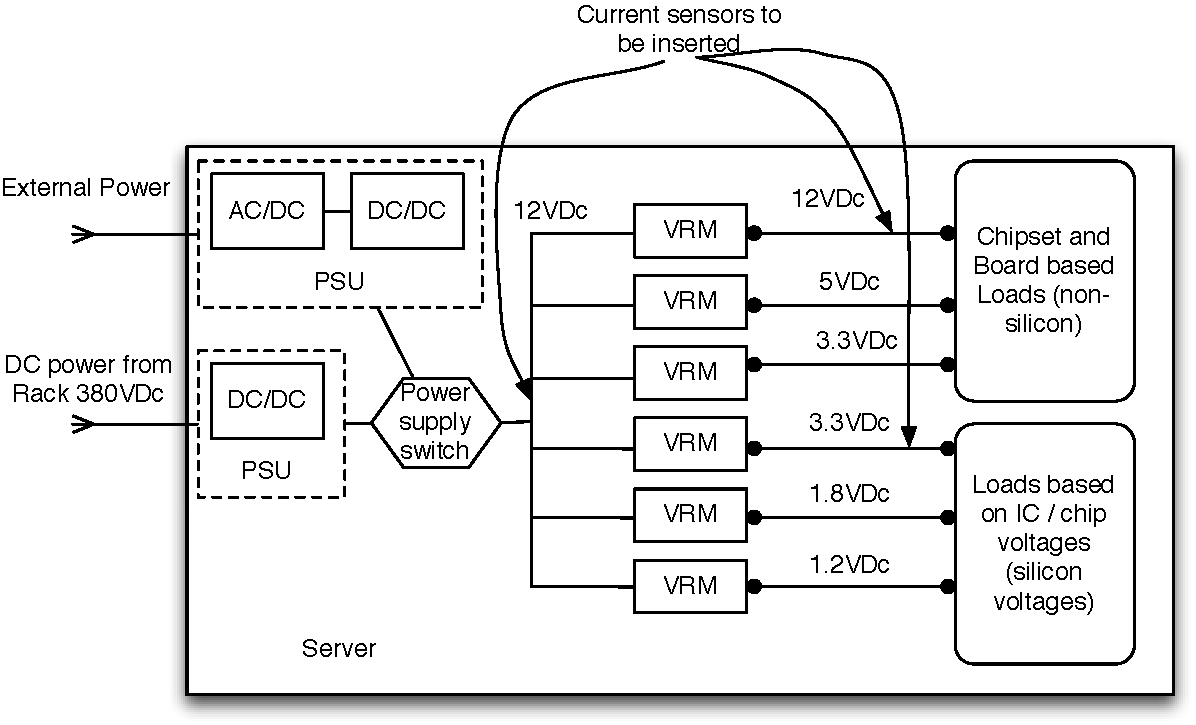
\includegraphics[scale=0.50]{acdcpower2.pdf}
\caption{Power distribution model for the server blade}
\label{fig:acdcpwr}
\end{center}
\end{figure}

Therefore, a rack level DC power distribution system easily translates
into large power savings at the server level.  We only consider a part
of this power conversion unit as part of our model as it is not software
tunable in its present sate at the level considered within this
work. However, current sensors, for example using MAXIM's 4473
\cite{maxim2006}, at the outputs from the power supply as performance
counters would immensely aid in dynamically tracking DC power draw into
the system which varies according to the system load.  Our aim through
this model is to monitor this input power to the system and control the
power and consequently thermal envelope of the system based on the
processing load. A proposed system diagram for a combined AC and DC
power-supply based system with performance counter measurable current
sensors, along with power distribution, is shown in figure
~\ref{fig:acdcpower}

\begin{figure}[ht]
  \begin{minipage}[b]{0.5\linewidth}
     \centering
     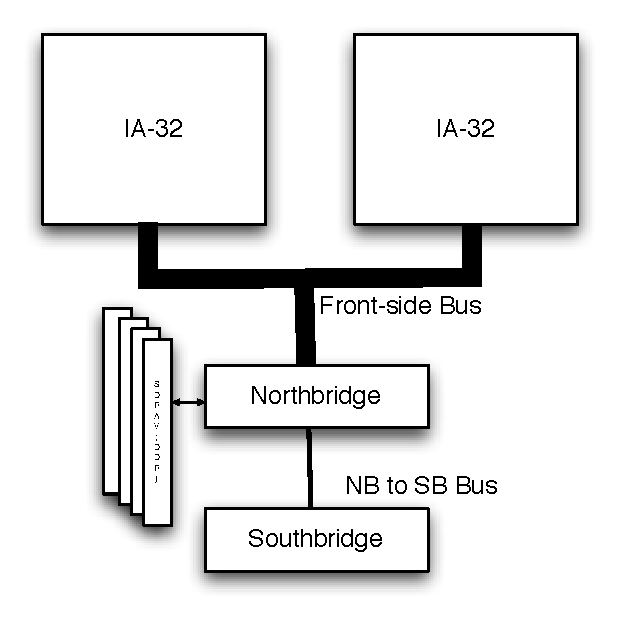
\includegraphics[scale=0.50]{intelarch.pdf}
     \caption{Intel Core Server Architecture}
     \label{fig:intarch}
   \end{minipage}
   \hspace{0.5cm}
   \begin{minipage}[b]{0.5\linewidth}
     \centering
     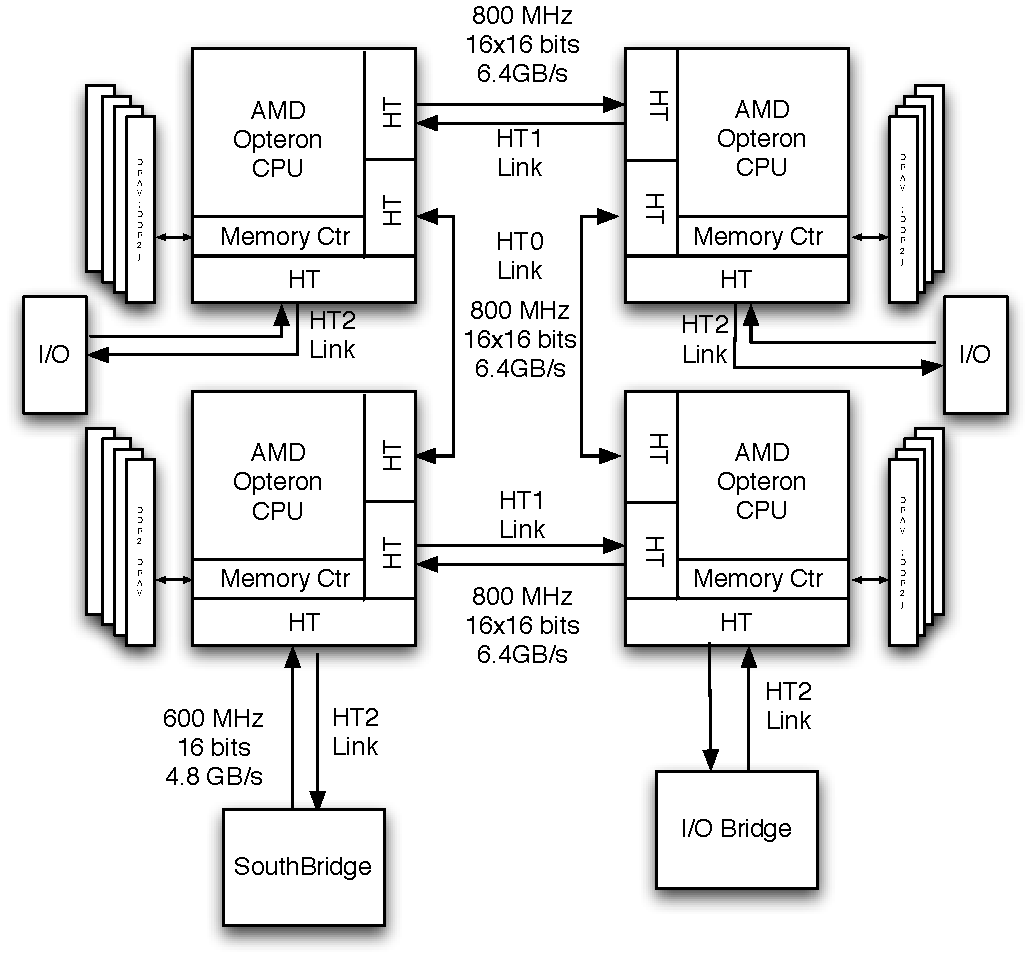
\includegraphics[scale=0.50]{amdhtarch1.pdf}
     \caption{AMD Opteron Server Architecture}
     \label{fig:amdarch}
   \end{minipage}
\end{figure}

In order to develop an energy consumption model based on computational
computational load of the system, we begin by measuring the total DC
power input to the system, at the output of the SMPS. As mentioned
earlier, the DC power is delivered in domains of +/-12 V, +/-5V, and +/-
3.3V. Most SMPS will limit the total power delivered through the 5V and
3.3V lines to about 20\% of the rated power supply ($P_R$). Now assuming
each of the voltage lines $v_k(t)$ draws current $i_k(t)$, then each
line draws an instantaneous power $p_k(t) = v_k(t)\cdot i_k(t)$. If a
voltage domain has $M$ DC lines as output, then total power delivered
for that voltage domain is :
  
\begin{equation}
\label{eq:power_vdomain}
p_{v1}(t)=  \sum_{k=0}^{M} v_k(t)\cdot i_k(t)
\end{equation}

If the board has $N$ voltage domains, then the total DC power delivered
into the system is :

\begin{equation}
\label{eq:power_vtot}
p_{dc}(t) = \sum_{j=0}^{N} p_{vj}(t)=  \sum_{j=0}^{N} \sum_{k=0}^{Mj} v_{k}(t)\cdot i_{k}(t)
\end{equation}

So total energy delivered to the system between times $t_2$ to $t_1$ is :

\begin{equation}
\label{eq:energy_vtot}
E_{dc} = \int_{t_1}^{t_2} p_{dc}(t) dt = \int_{t_1}^{t_2} \sum_{j=0}^{N} p_{vj}(t) dt = \int_{t_1}^{t_2} \sum_{j=0}^{N} \sum_{k=0}^{Mj} v_{k}(t)\cdot i_{k}(t) dt
\end{equation}

For the 3.3V and 5V lines thus, the following constraint holds :

\begin{equation}
\label{eq:power_constr}
E_{dclv} = \int_{t_1}^{t_2} p_{dclv} (t) dt =  \int_{t_1}^{t_2} ( \sum_{k=0}^{M1} v_{k}(t)\cdot i_{k}(t) + \sum_{k=0}^{M2} v_{k}(t)\cdot i_{k}(t) ) dt  \leq 0.2 P_R
\end{equation}

where $M1$ and $M2$ are the total 3.3V and 5V lines respectively. Thus in our 450W rated system the power
delivered by the 3.3V and 5V lines is capped at 90W. 

This energy delivered to the system $E_{dc} = E_{system}$ can now be
expressed as a sum of energies consumed by the different sub-systems in
the server blade.  Broadly we define five sources of energy consumption
within a system:
\begin{itemize}
\item $E_{proc}$: Energy consumed in the processor due to all
  computations
\item $E_{memory}$: Energy consumed in the DRAM chips and
\item $E_{em}$: Energy consumed by all electrical and electromechanical
  components in the server blade.  This includes fans, and other
  components on the server which consume AC power.
\item $E_{board}$: Energy consumed by perphierals that support the
  operation of the board. These include all devices in the multiple
  voltage domains across the board, in cluding chipset chips, voltage
  regulation, bus control chips, connectors, interface devices etc.
\item $E_{hdd}$: Energy consumed by the hard disk drive during the
  server's operation.
\end{itemize}

We explore each of these terms in turn by following an energy
conservation model in the system.  In order to a get a true measure of
the computational load on the system, our method looks to snoop on
completed bus transactions per unit time in the system and measure the
relative change in energy consumption (as indicated by change in
temperature) as computation tasks are completed.  Use of this
performance counter metric as compared to other metrics fits well with
the architecture of microprocessors used in NUMA-based processors in
multicore environments.

Consider the Intel Pentium and AMD Operton processor architectures
connected in a dual core configuration shown in
Figures~\ref{fig:intarch} and ~\ref{fig:optarch}.  The Pentium
architecture (and its successors) is based upon the idea of a
Front-Side-Bus (FSB) which connects individual cores to the Northbridge
chip.  This chip provides the interface between the cores and memory.  A
coherent bus protocol is used to ensure consistency in memory access
between the cores.  For this architecture, the FSB becomes a performance
bottleneck as processor and cores have to moderate themselves to the
slower speed of the bus.

Contrast this with the NUMA-based architecture used by the AMD Opteron (Figure~\ref{fig:amdarch}).  
In this case, the Northbridge functionality is combined
onto the same processor die as each core and each core is responsible for
local access to the memory connected to that Northbridge. Cores on a single
die are connected via a crossbar to the Hypertransport bus between
processors.  Again, a coherent bus protocol is used to ensure memory
consistency between cores and processors. In addition, the master processor
in the system is connected via a second Hypertransport bus to the Southbridge
device that manages connections to the outside world.

We see that the work done by any of these processors, which is at the
heart of energy consumption in a server system, can be quantified in
terms of bus transactions in and out of these processors.  The traffic
on the external buses give us a measure of how much data is being
processed by the processor and what would be an upper limit of the work
done by a single processor. In our approach we concentrate on developing
the energy consumption model on a Hypertransport (HT) based system with
two AMD dual core Opterons in a Sunfire X2200 server.

\subsection{Modeling Processor energy consumption}
\label{sec:procmodel}

In previous work, processor power consumption has been based on
computing the activity based based power in a processor.  In a
processor, during computation, as the processor executes its sequence of
instructions and operates on the given data, energy is consumed due to
the amount of switching activity taking place within a processor. From
an IC design standpoint, this energy consumption per unit time is
broadly given by :

\begin{equation}
\label{eq:power_proc}
P_{processor}=  \alpha*C*V_{dd}^2*f + I_{static}*V_{dd} + V_{dd}*I_{leakage}
\end{equation}

where $\alpha$ is the switching activity in the first term which is the
\emph{dynamic power consumption}, $V_{dd}$ is the supply voltage, $C$ is
the total associated capacitance, $I_{static}$ is the static current
flowing when there is no activity (switching), and $I_{leakage}$ is the
leakage current due to low threshold voltages in the processor. In
general, the attempt is to reduce the first term, as it is the dominant
energy consuming term in the equation. Besides reducing the operating
voltage, clock frequency and total chip capacitance, a lot of
architectural effort goes into reducing $\alpha$ which is known as the
\emph{activity factor}, or in other words, the switching probability.

However with the complexities of today's chips and far more complex
chips to come, getting a real-time, estimate of this switching activity
on silicon is infeasible. Though an IC designer could do it, but in a
server system, in real-time, getting switching based power on silicon
would require a lot of computational effort. DVFS (dynamic frequency and
voltage scaling) techniques are currently applied to control the first
term in the power equation, which works well since the voltage and
operating frequency are dominant components in the power
consumption. However to predict $\alpha$ for load-based power
consumption is very hard.

We approach the processor power consumption issue from an energy
conservation standpoint.  If we consider the processor a closed energy
system, then based on the input and the output to the processor, we
could model its energy workload in measurable terms. Also, to have
real-time measures of the energy consumed by the processor, we need to
develop our model in terms of observable performance counters in the
system. In order to do that, We focus on measuring the bus activities on
the system wide buses which transport data to and from the processors as
they operate (in this case the traffic on the HT buses), as given by the
utility \texttt{cpustat}. We are also able to measure the thermal
consequences of the work done by the processor by measuring CPU die
temperature and ambient temperature using the utility \texttt{ipmi}.

Focusing on the system at hand, the HyperTransport standard specifies
that the energy consumed per bit of the



The first task in estimating the power consumption of a digital system
is to identify the typical application programs that will be executed on
the system. A non-trivial application program consumes millions of
machine cycles, making it hard to get power estimate for a particular
application. In \cite{Sato1995} the power cost of a CPU module is
characterized by estimating the average capacitance that would switch
when the CPU module is activated. In \cite{Su1994} , the switching
activities on buses (address, instruction, data) are used to estimate
the power consumption of the microprocessor. In \cite{Tiwari1994}, based
on actual current measurements of some processors, the following
instruction-level power mode is proposed:

\begin{equation}
\label{eq:power_prog}
E_{program}=  \sum_i (BC_i*N_i) + \sum_{i,j} (SC_{i,j}*N_i) + \sum_k (OC_k)
\end{equation}
 
is the total energy dissipation of the program which is divided into
three parts. The first part is the summation of the base energy cost of
each instruction $BC_i$ is the base energy cost and $N_i$ is the number
of times instruction $i$ is executed. The second part accounts for the
circuit state $SC_{i,j}$ is the energy cost when instruction $i$ is
followed by $j$ during the program execution. Finally, the third part
accounts for energy contribution $OC_k$ of other instruction effects
such as stalls and cache misses during the program execution.
 
We attempt to extend the concept of measuring power by measuring
switching activities and tasks completed on buses at various levels in
the system, as an indicator of the computational work done by the
system, and we try to develop an energy consumption and thermal model of
the system based on activities on the buses.

The energy consumed by the system for a given computational worklaod is
modeled as a function of these metrics:

\begin{equation}
\label{eq:linmodel}
E_{system}=  A*E_{proc}+B*E_{memory}+C*E_{em}+D*E_{board}+F*E_{hdd}
\end{equation}

where $A$,$B$,$C$, and $D$ are unknown constants to be determined. 

The AMD processor used in our case study has a unified Level 2 cache
shared amongst each core in the processor.  The cost of accessing this
memory can be calculated using the following formula:
\begin{equation}
  \label{eq:Level1cost}
  insert equation here
\end{equation}

The calculation of data access energy cost is complicated by the use of
the NUMA architecture.  The AMD Opteron family of processes provides a
single, unified view of memory; however, as shown in Figure
\ref{fig:optarch}, each processor in the system manages a bank of the
physical memory.  As such, There are two cases to be considered for
memory access:
\begin{itemize}
\item the memory is local to the processor
\item the memory location is physically attached to a remote processor
\end{itemize}
In the first case, the method used to access the memory works in the
traditional manner and the energy cost is calculated as
\begin{equation}
  \label{eq:Level1cost}
  insert equation here
\end{equation}
\begin{figure}
  \centering
  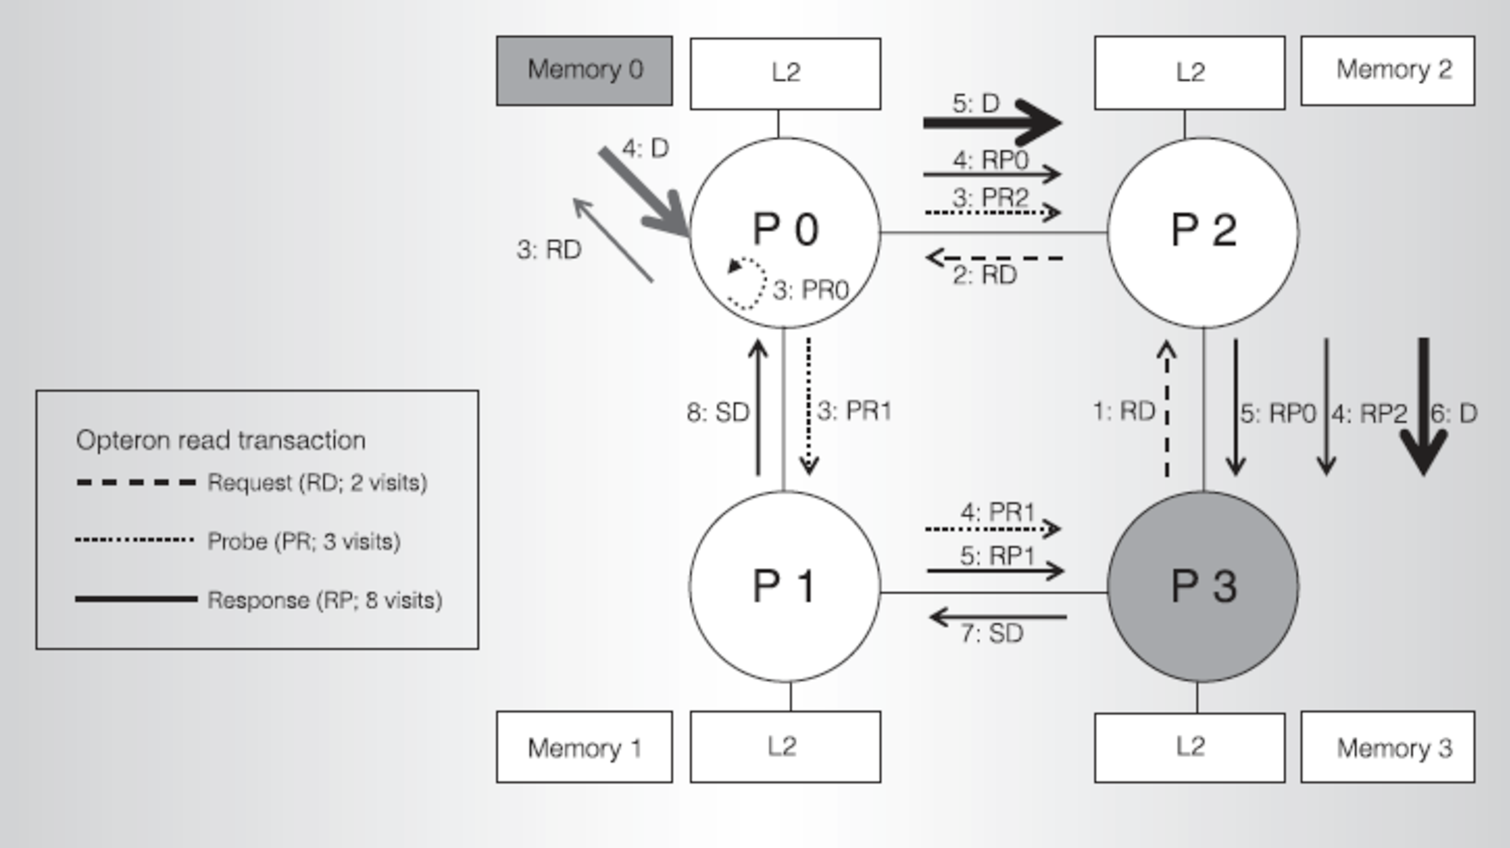
\includegraphics[scale=0.50]{amdoptcht.pdf}
  \caption{Example of a remote memory transaction on the AMD Opteron \cite{amd2004}}
  \label{fig:amdcht}
\end{figure}
For the case where a CPU core attempts to access a memory location that
is located on another physical processor, then the equations for
calculating the energy cost must take into account the energy cost for
the Hypertransport bus traffic.   Consider the example of a 4-processor
configuration shown in Figure \ref{fig:amdcht}.  In this case if a CPU
core on processor 0 attempts to access memory connected to processor 3,
up to seven bus transactions are required to access to process the read
request and ensure memory coherency.

Taking this into account, we need to first consider the energy cost of a
single transaction on the cHT bus.  This can be calculated using the
following formula:
\begin{equation}
\label{eq:singelHTcost}
insert equation here
\end{equation}

Then, considering the case of the read transaction shown in Figure
\ref{fig:amdcht}, the energy cost of a read transactions is
Similarly, an attempt to performm a write transaction results in the
following eneregy cost:


\subsection{Hard disk energy}
\label{sec:networkengery}
The energy consumed by the hard disk while operating can be estimated in
a couple of ways. Though neither of the methods are exact, they give an
upper bound on the energy consumption of the hard disk when jobs are
running on the server blade. In our server, Hitcahi's 7200 RPM 250G,
SATA hard disk is used. Table ~\ref{tab:hddparam} lists the typical
power consumption numbers for the hard disk used. Based on the physical,
electrical and electromechanical parameters of the hard disk, very
detailed power consumption models can be constructed. However we can
achieve a cruder but simpler model based on the typical power
consumption data of the hard disk and performance counters.

\begin{table}[h!t!]
\caption{HItachi HDT725025VLA360 disk power parameters}
\begin{tabular}{ l l }
\hline 
\hline
Parameter & Value \\
\hline
  Interface & Serial ATA  \\
  Capacity & 250 GB  \\
  Rotational speed & 7200 rpm  \\
  Power (spin up) & 5.25 W (max)  \\
  Power (Random read, write) & 9.4 W (typical)  \\
  Power (Silent read, write) & 7 W (typical)  \\
  Power (idle) & 5 W (typical)  \\
  Power (low RPM idle) & 2.3 W (typical for 4500 RPM)  \\
  Power (standby) & 0.8 W (typical)  \\
  Power (sleep) & 0.6 W (typical)  \\
\hline \hline
\end{tabular}
\label{tab:hddparam}
\end{table}

The utility \texttt{iostat} can be used to measure the number of read
and writes per second to the disk as well as the kilobytes read from and
written to the disk. Thus based on this performance counter, we can
compute an approximate disk power consumption $E_{hdd}$ value as :

\begin{equation}
\label{eqn:hddpwr1}
E_{hdd} = P_{spin-up}\times T_{su}  +  P_{read}\sum N_r\times T_r + P_{write}\sum N_w\times T_w + \sum P_{idle}\times T_{id}
\end{equation}

where $P_{spin-up}$ is the power required to spin-up the disk from 0 to
full rotation. $T_{su}$ is the time required to achieve spin
up. $T_{su}$ is typically about 10s. $P_{read}$ is the power consumed
per kilobyte of data read from the disk. $N_r$ is the number of
kilobytes of data read in time-slice $T_r$ from the disk. The variables
are analogous for the write energy consumption. $P_{read}$ for our
Hitachi disk can be computed as follows:

The read operation at 1.5 Gbits/s consumes 530 mA current at +5V. Hence
every kilobyte read, consumes approximately $13.3 \mu
W$/Kbyte. Similarly, every write operation consumes $6.67 \mu
W$/Kbyte. The numbers $N_r$ and $N_w$ can be obtained using
\texttt{iostat} and out choice of time-slice.

The idle state has two conditions, idle and unloaded idle, where in the
latter case the heads are unloaded. The time to go from unloaded to idle
is usually less than 1 second, which is less than the resolution of
\texttt{iostat}. Thus, a history match count in the \texttt{iostat}
statistics where the reads and writes have been zero, tells us the
period in which the disk is idle, and the idle energy consumption can be
computed accordingly. \texttt{iostat} reading based conditions for
switching to different disk power states can be obtained with more
in-depth analysis, but the net results falls into this equation's
framework. That analysis is the topic of a future work.

The hard disk power can also be measured in real-time if current sensors
are provided at the output of the DC voltage lines delivering power to
the hard disk drives. The +5V lines will draw a maximum current of 730mA
and the +12V lines will draw a maximum current of 630mA. Thus $E_{hdd}$
can also be formulated as :

\begin{equation}
\label{eqn:hddpwr2}
E_{hdd} =  \int_{t1}^{t2} \left \{ v_1(t)\times i_1(t) + v_2(t)\times i_2(t) \right \} dt
\end{equation}

This approach can be applied in the presence of current sensors which in
our experiments we measured with a current probe and logged through an
oscilloscope.

\subsection{Board Components}
\label{sec:board}
The quantity $E_{board}$ captures the energy dissipated by the need to
power supporting components on the board.  This quantity takes into
account power consumed by active cooling devices (fans, water cooling)
and is calculated by

\subsection{Electromechanical Energy}
\label{sec:electrical}
There is a basic electrical cost related to running the computer. The
quantity $E_{elect}$ in our model takes these quantities into account.
$E_{elect}$ is calculated as summation of the DC and AC power
consumption in the peripherals supporting the processor, particularly
the electromechanical components. This is mainly the power cosumption in
the power supply unit and the power consumption in the cooling fans.
As discussed earlier, the AC to DC conversion process is a load based number and
has a best case conversion efficiency of 80\% and a nominal efficiency of 75\% .

Power drawn by the fans for cooling can be given by the following equation:

\begin{equation}
\label{eq:fanp}
P_{fan}=  P_{base} \cdot (\frac{RPM_{fan}}{RPM_{base}})^3
\end{equation} 

$P_{base}$ in this case defines the base of the unloaded system. In our
case, that is the power consumption of the system when running only the
base operating system and no other jobs. That value is obtained
experimentally by measuring the current drawn on the +12V and +5V lines,
using a current probe and an oscilloscope. There is a current surge at
system startup, which is neglected and under nominal conditions, the
+12V line draws approximately 2.2A, which powers both teh blowers fans
in the system. The two peripheral fans running at +5V draw around 2.1A
of current.  Thus the base power for the fans in known.  IPMI sensors
easily collect fan RPM data, and hence it is possible to quantify the
electrical power consumption in the system. Thus the electrical power
consumption can be quantified as:

\begin{equation}
\label{eq:elect}
P_{elect}=  V(t) \cdot I(t) + \sum_{i=1}^NP_{i}
\end{equation} 

where the first term in the equation is the instantaneous DC power
output from the power supply and is the DC power consumed by the
system. $N$ is the number of fans in the server and $P_{i}$ is the
instantaneous power consumed by the $i-th$ fan according to equation
~\ref{eq:fanp}. 

\begin{equation}
\label{eq:elect}
\eta=  \frac{V(t) \cdot I(t)}{P_{in}}
\end{equation} 

$\eta$ gives a measure of the energy conversion efficiency, into the
system from the mains, and gives an idea of the energy budget available
to the system.

Thus the total energy consumption during a given task period $T_{p}$ due
to electrical energy in the system can now be given by:

\begin{equation}
\label{eq:elect}
E_{elect} =  \int^{T_{p}}_0 [V(t) \cdot I(t) + \sum_{i=1}^NP_{i}]\,dt
\end{equation} 

\subsection{Putting it all together}
\label{sec:wholemodel}


\section{Experimental Study}
\label{sec:experiment}
We have performed an experimental study of our model's behavior to answer the
following questions:
\begin{itemize}
\item 
  What are the coefficients in the linear regression equation that
  correlates power with bus transactions, CPU die temperature, and
  ambient temperature?
\item What is the accuracy of our general model compared against
  observed power consumption during the execution of a set of CPU benchmarks?
\end{itemize}
\subsection{Experiment Environment}
\label{sec:expdesign}
\begin{table}
  \centering
  \label{tab:hardware}
  \begin{tabular}{l|l}
    \hline
    &\textbf{Sun v20s}\\  
    \hline 
    CPU&2 AMD Opteron K10 Processors\\
    \hline 
    CPU L2 cache&2x2MB\\
    \hline 
    Memory&8GB\\
    \hline 
    Internal\\disk&250GB\\
    \hline 
    Network\\ Interface Card&4x1000Mbps\\
    \hline 
    Video&On-board \\
    \hline 
    Height&1 rack unit\\
    \hline
  \end{tabular}
  \caption{Test Hardware Configuration}
\end{table}
The test hardware used to evaluate our model is a Sun Fire X2200 server
configured as shown in Table \ref{tab:hardware}.

The power consumed is measured with a WattsUP \cite{WattsUp2006a} power
meter connected between the AC Main and System Under Test (SUT).
The power meter measures the total and average wattage, voltage, and
amperage over the run of a workload.  The internal memory of the power
meter is cleared at the start of the run and the measures during the run
are downloaded after the run completes from the meter's internal memory
into a spreadsheet \cite{WattsUp2006b}.

Current flow on the different voltage domains in the server is measured
using an Agilent MSO6014A oscilloscope with one or more Agilent 1146A current
probes.  The current probes magnetically measure the current flowing
through the 12v, 5v, and 3.3v connections provided by the server power
supply.  This data is collected from the oscilloscope at the end of the
execution of a benchmark and stored in a spreadsheet on the test host.

Four classes of metrics are sampled at 5 second intervals during the
experiment:
\begin{itemize}
\item CPU temperature (for all processors in the system)
\item Ambient temperature in the computer case (measured in one more
  locations using the sensors provided by server manufacturer)
\item The number of completed transactions processed through the system bus
\end{itemize}
System data is collected from the system baseboard controller using the
IPMI interface. Processor performance counters are collected on a
system-wide basis using the Solaris \texttt{cpustat} utility.

\subsection{Experimental Derviation of Power Model}
\label{sec:model}
\begin{table}
  \centering
% Table generated by Excel2LaTeX from sheet 'ByBenchmark'
\begin{tabular}{|r|r|r|r|r|r|r|r|r|r|r|}
\hline
           &      bzip2 & catctusADM &     gromac &    h264ref &        lbm &    leslie3 &        mcf &    omnetpp &  perlbench &     povray \\
\hline
\hline
           & -454.34694 & -452.70875 & 2389.74716 &  -212.6751 & 102.408099 & -890.39441 & -241.07685 &  1513.1436 & -265.92096 & 162.159281 \\
\hline
Ambient\_Temp0 &  37.353369 &   8.917419 &   9.478305 &  13.470463 &  -1.567693 &  -0.938896 &   7.805745 & -145.11964 &  -5.839846 &   2.385918 \\
\hline
Ambient\_Temp1 &  -0.710206 &  12.122969 & -92.167692 &  -0.348331 &    7.24114 &  -0.006705 &   3.694106 & -54.494823 &  28.326739 &  12.592825 \\
\hline
CPU\_0\_Temp &   8.390433 &  -0.411644 &  -5.991155 &   -0.46091 &  -9.464558 &  15.664689 &   3.362209 &  -7.125749 &  -1.224856 &  -2.990661 \\
\hline
CPU\_1\_Temp &  -12.83983 &   3.463641 &  -9.947242 &   2.284206 &    1.06833 &  26.833784 &   0.622109 &  99.090608 &  -8.558473 & -15.748618 \\
\hline
       HT1 &   0.362642 &     0.4787 &   4.150526 &   0.264177 &  -0.458475 &  -2.186466 &   0.038969 &   2.320652 &    0.92799 &   0.302935 \\
\hline
       HT2 &  -0.243124 &  -0.297717 &  -1.924114 &  -0.738151 &   0.655436 &   0.965717 &  -0.090382 &  -3.250674 &   -0.97342 &  -0.393772 \\
\hline
Interaction Terms: &  -0.627386 &  -0.282452 &   0.643871 &   0.022666 &  -0.122164 &    0.20859 &  -0.185486 &   1.178204 &  -0.711443 &  -1.020471 \\
\hline
           &  -0.439677 &   0.011435 &  -0.685264 &  -0.139129 &   0.087435 &    0.05187 &   -0.04928 &   1.028112 &   0.046473 &  -0.048759 \\
\hline
           &   0.156305 &    0.06779 &  -0.158503 &  -0.184729 &   0.068367 &  -0.240718 &   0.047329 &   1.122329 &   0.718588 &   0.935815 \\
\hline
           &   0.015841 &   0.040063 &   0.001284 &   0.010041 &   0.009801 &   0.021047 &   0.006005 &   0.072324 &  -0.043823 &   0.026955 \\
\hline
           &   0.002618 &  -0.025119 &   0.039915 &   0.034548 &  -0.014028 &  -0.010606 &  -0.006471 &  -0.119235 &   0.053837 &     0.0027 \\
\hline
           &   0.250014 &   0.050268 &   0.906605 &   0.012081 &   0.066504 &  -0.078387 &   0.038796 &   1.588699 &   0.163604 &   0.523678 \\
\hline
           &   0.246089 &   -0.10046 &   0.539212 &  -0.039526 &   -0.11117 &  -0.060244 &   0.027079 &  -1.111383 &  -0.195768 &   0.016859 \\
\hline
           &  -0.000103 &   0.041005 &  -0.081099 &   0.015508 &  -0.000062 &  -0.001763 &   -0.00769 &   -0.04217 &   0.007076 &  -0.018375 \\
\hline
           &  -0.002883 &  -0.023746 &  -0.000768 &  -0.079378 &  -0.000392 &  -0.001416 &   0.010914 &   0.077967 &  -0.010993 &    0.03437 \\
\hline
           &  -0.063158 &  -0.028859 &  -0.200348 &   0.132611 &   0.050153 &  -0.336107 &  -0.075903 &  -2.095991 &  -0.159396 &   -0.39047 \\
\hline
           &  -0.013073 &  -0.028254 &   0.021246 &  -0.024003 &   0.012842 &   0.051658 &   0.010662 &  -0.069699 &   0.011561 &  -0.027141 \\
\hline
           &   0.004447 &   0.014493 &  -0.022502 &   0.070095 &  -0.016234 &  -0.022645 &  -0.014669 &   0.098471 &  -0.010591 &  -0.002605 \\
\hline
           &  -0.006558 &  -0.049482 &  -0.027981 &  -0.003864 &  -0.007802 &  -0.014011 &  -0.007053 &   0.000253 &  -0.004575 &   0.016814 \\
\hline
           &   0.001945 &   0.032753 &   0.032236 &   0.002916 &   0.010156 &   0.009455 &   0.009469 &  -0.005405 &   0.002303 &  -0.025138 \\
\hline
           &  -0.000049 &  -0.000044 &  -0.000758 &  -0.006849 &  -0.000007 &  -0.000084 &   -0.00003 &  -0.000041 &  -0.000362 &   0.001268 \\
\hline
     R-sq: &   0.951341 &   0.970471 &   0.952007 &   0.947114 &    0.96882 &   0.906724 &   0.959689 &   0.931247 &   0.953341 &   0.923945 \\
\hline
Adj. R-sq: &  0.9568393 &   0.968812 &   0.948818 &   0.944273 &   0.966917 &    0.89947 &   0.957692 &   0.926937 &    0.95025 &   0.917249 \\
\hline
\end{tabular} 
  \caption{Power Regression Model for Each Benchmark}
  \label{tab:bybench}
\end{table}
Our first set of experiments has two purposes: characterize the power 

\subsection{Model Verification}
\label{sec:linearreg}


\section{Discussions}
\label{sec:conclusions}
The model developed in this paper would hold well for any dual-core
opteron based dual-processor system using the HyperTransport system
bus. However it is scalable easily to a quad-core dual processors
opteron system using HyperTransport. One would expect to see a slight
difference or variation in the predicted power due to the greater or
diminished affect of the die temperatures on the other parameters and
the model would have to be adjusted accordingly. For a dual-core
quad-processor system, the additional HT0 term would be introduced
into the CPU power consumption term and the
$\beta$ coefficients would have to be recalculated, and the cpu power
will have more terms. For a quad-core quad processor system, similar
recalculations would be required.

Though the computations have not yet been done on INTEL's Xeon
platforms, the computation methodology holds for those platforms too.
Instead of measuring the HT0 through HT2 traffic for the Xeon, we would
primarily measure performance counters like \texttt{BUS\_TRANS\_ANY},
\texttt{BUS\_TRANS\_MEM}, and \texttt{BUS\_TRANS\_BURST}.  Similar model
development and coefficient extraction arguments would hold for dual and
quad core Xeons in different processor configurations. Currently without
data from the INTEL processors it is hard to say wether the more is more
accurate on a certain platform as compared to the other.

Besides these two processors, other major processors used in large
data centers are SUN's T1 and T2 (Niagara) processors which also use
HyperTransport for external system bus communications. There are more
enhanced performance counters on those processors for monitoring bus
activity and power and temperature control. All major HPC and
data-center processor providers and support chip providers support
Hypertransport and it is reasonable to argue that for any other
processor (FPGA based , custom ASIC etc.) which supports system bus
monitoring performance counters, a similar methodology can be
employed to develop a real-time power model.

In terms of measuring th performance counters, we have used Solaris 10
utilities \texttt{cpustat}, \texttt{iostat}, and \texttt{ipmi}. Of these
\texttt{ipmi} and \texttt{iostat} are available across all operating
systems, Linux, Solaris, MacOS X or any other operating system used in
data centers. \texttt{cpustat} is a Solaris specific utility but is
already being ported to Linux. \texttt{mpstat} is not used since even
though it is geared towards multiprocessor systems, does not give a good
measure of inter-processor bus transactions. In future work, it is
planned to use tools like \texttt{dtrace} and \texttt{oprofile} for more
controllable and tunable performance parameters which have major impacts
on system-wide and processor wide power consumption.

\section{Conclusions and Future Work}
\label{sec:conclusions}

\label{sec:references}
\nocite{*}
\bibliographystyle{latex8}
\bibliography{infotheory.bib}



\begin{table}
  \centering
  \begin{tabular}{l|l||l}
    $Time$&$Predicted$&$Actual$\\
    \hline
    5 & xxx & xxx\\
    20& xxx & xxx\\
  \end{tabular}
  \caption{Experiment 2: Model Prediction versus Actual On Idle System}
  \label{tab:exp2design}
\end{table}

\begin{table}
  \centering
  \begin{tabular}{l|ll}
    &Master Model&Predictive Model \\
    $RMSE$&108.084&107.538\\
    $R-square$&48.06\%&45.15\% \\
    $Adjusted R-square$&41.13\%&41.72\% \\
    $Coefficient of variation$&3.301832&3.285167 \\
  \end{tabular}
  \caption{Fit Statistics for Experiment 2}
  \label{tab:exp2fit}
\end{table}

\begin{table}
  \centering
  \begin{tabular}{llllll|lllll}
    \multicolumn{1}{c}{} & \multicolumn{5}{c|}{Master Model}&\multicolumn{5}{c}{Predictive Model} \\
    Source&$DF$&$MS$&$MS$&$F$&$PR>F$&$DF$&$SS$&$MS$&$F$&$Pr>F$ \\
    \hline
    $IFP$&1&152325.300&152325.300 &13.0392&0.00257&1&152325.300&152325.300&13.172&0.002255 \\
    $WXEN$&1&9800.000&9800&0.839&0.374&&&&& \\
    &&&&&&&&&& \\
    $Model$&2&162125.300&81062.670&6.939065&0.00735&1&152325.300&152325.300&13.1719&0.00226\\
    $Error$&15&175231.100&11682.070&&&16&185031.100&11567.440&&\\
    $(Lack of Fit)$&3&52207.110&17402.370&1.975&0.220&1&22002.780&22002.780&2.0244&0.1753\\
    $Total$&17&337356.400& & & &17&337356.400&&& \\
  \end{tabular}
  \caption{ANOVA Analysis for Experiment 2}
  \label{tab:exp2anova}
\end{table}


\end{document}

